\documentclass[12pt,letterpaper]{article}
\usepackage[spanish,es-nodecimaldot]{babel}
\usepackage[utf8]{inputenc}
\usepackage[T1]{fontenc}
\usepackage{geometry}
\usepackage{graphicx}
\usepackage{amsmath}
\usepackage{float}
\usepackage{booktabs}
\geometry{margin=2.5cm}
\graphicspath{{figuras/}}

\title{Cálculo de una trayectoria individual de simulación Monte Carlo para el precio del oro}
\author{Alejandro Ramirez \and Leidy Paola Patiño}
\date{\today}

\begin{document}
\maketitle

\section{Propósito}
Este documento explica cómo el código generó una sola trayectoria simulada del precio del oro bajo el escenario base. La trayectoria no representa el pronóstico único del modelo, sino una posible realización aleatoria dentro del conjunto de simulaciones Monte Carlo.

\section{Modelo utilizado}
La trayectoria fue generada con el modelo final seleccionado por el flujo mejorado: \textbf{LightGBM optimizado con Optuna}. Este modelo fue elegido porque obtuvo el menor RMSE promedio en validación temporal. En la etapa anterior del trabajo se había seleccionado XGBoost por menor error, pero la comparación ampliada mostró que LightGBM con búsqueda automática de hiperparámetros mejoró el desempeño de validación.

El modelo se entrenó con la variable objetivo:
\begin{equation}
r_{t+1}=\ln\left(\frac{P_{t+1}}{P_t}\right),
\end{equation}
y posteriormente cada retorno predicho se transformó a precio mediante:
\begin{equation}
\hat{P}_{t+1}=P_t e^{\hat{r}_{t+1}}.
\end{equation}

\section{Precio inicial}
La simulación parte del último precio observado en la base histórica, que fue aproximadamente:
\begin{equation}
P_0=4719.285\;\text{USD/oz}.
\end{equation}

\section{Retorno base del modelo}
Para cada fecha futura, el modelo de machine learning estima un retorno logarítmico base:
\begin{equation}
\hat{r}_t=f(X_t),
\end{equation}
donde $X_t$ contiene rezagos, retornos, medias móviles, volatilidad, variables de plata, precios NI y variables macroeconómicas disponibles.

\section{Choque aleatorio}
La trayectoria individual no usa únicamente el retorno base. Se agrega un choque aleatorio:
\begin{equation}
u_t=\phi u_{t-1}+\sqrt{1-\phi^2}z_t,
\end{equation}
donde $z_t\sim N(0,1)$ y $\phi$ controla la persistencia de los choques. Para el escenario base se usó una persistencia moderada.

En el escenario base, el código usó los siguientes parámetros de configuración Monte Carlo:
\begin{table}[H]
\centering
\caption{Parámetros de la simulación individual bajo escenario base.}
\begin{tabular}{lr}
\toprule
Parámetro & Valor \\
\midrule
Multiplicador de volatilidad & 1.00 \\
Probabilidad de salto diario & 0.004 \\
Media del salto & 0.0000 \\
Desviación del salto & 0.0045 \\
Persistencia de choques $\phi$ & 0.30 \\
\bottomrule
\end{tabular}
\end{table}

\section{Saltos aleatorios}
Además del choque normal, la simulación permite saltos ocasionales:
\begin{equation}
J_t=\begin{cases}
\eta_t, & \text{con probabilidad } p,\\
0, & \text{con probabilidad } 1-p.
\end{cases}
\end{equation}
Estos saltos representan eventos bruscos de mercado.

\section{Retorno simulado}
El retorno usado para la trayectoria individual fue:
\begin{equation}
r_t^{MC}=\hat{r}_t+u_t\sigma_s+J_t.
\end{equation}
En el archivo CSV también se guardó el choque neto:
\begin{equation}
\text{choque\_logret}_t=r_t^{MC}-\hat{r}_t.
\end{equation}

\section{Actualización del precio}
El precio se actualizó recursivamente:
\begin{equation}
P_t^{MC}=P_{t-1}^{MC}e^{r_t^{MC}}.
\end{equation}
Por esta razón la trayectoria puede subir o bajar respecto a la mediana. Si aparecen choques positivos consecutivos, la trayectoria toma una forma ascendente; si aparecen choques negativos, cae o se separa hacia abajo.

\section{Primera observación simulada}
En la primera fecha simulada, 2026-04-09, el retorno simulado fue aproximadamente $-0.01663$. Por tanto:
\begin{equation}
P_1^{MC}=4719.285\,e^{-0.01663}\approx 4641.44\;\text{USD/oz}.
\end{equation}
Esto explica la caída inicial de la trayectoria individual respecto al precio observado.

\section{Gráfica de la trayectoria}
La Figura \ref{fig:trayectoria} muestra la trayectoria única seleccionada. También se incluye la mediana del escenario base y la banda P10--P90 para comparar la trayectoria individual con el conjunto de simulaciones.

En la figura, los percentiles se leen así:
\begin{itemize}
    \item La banda sombreada inferior corresponde al percentil $P10$.
    \item La línea naranja corresponde al percentil $P50$, es decir, la mediana de todas las simulaciones.
    \item La banda sombreada superior corresponde al percentil $P90$.
    \item La línea roja corresponde a una sola trayectoria simulada. Esta trayectoria puede cruzar la mediana o acercarse a las bandas según los choques aleatorios que reciba.
\end{itemize}

\begin{figure}[H]
\centering
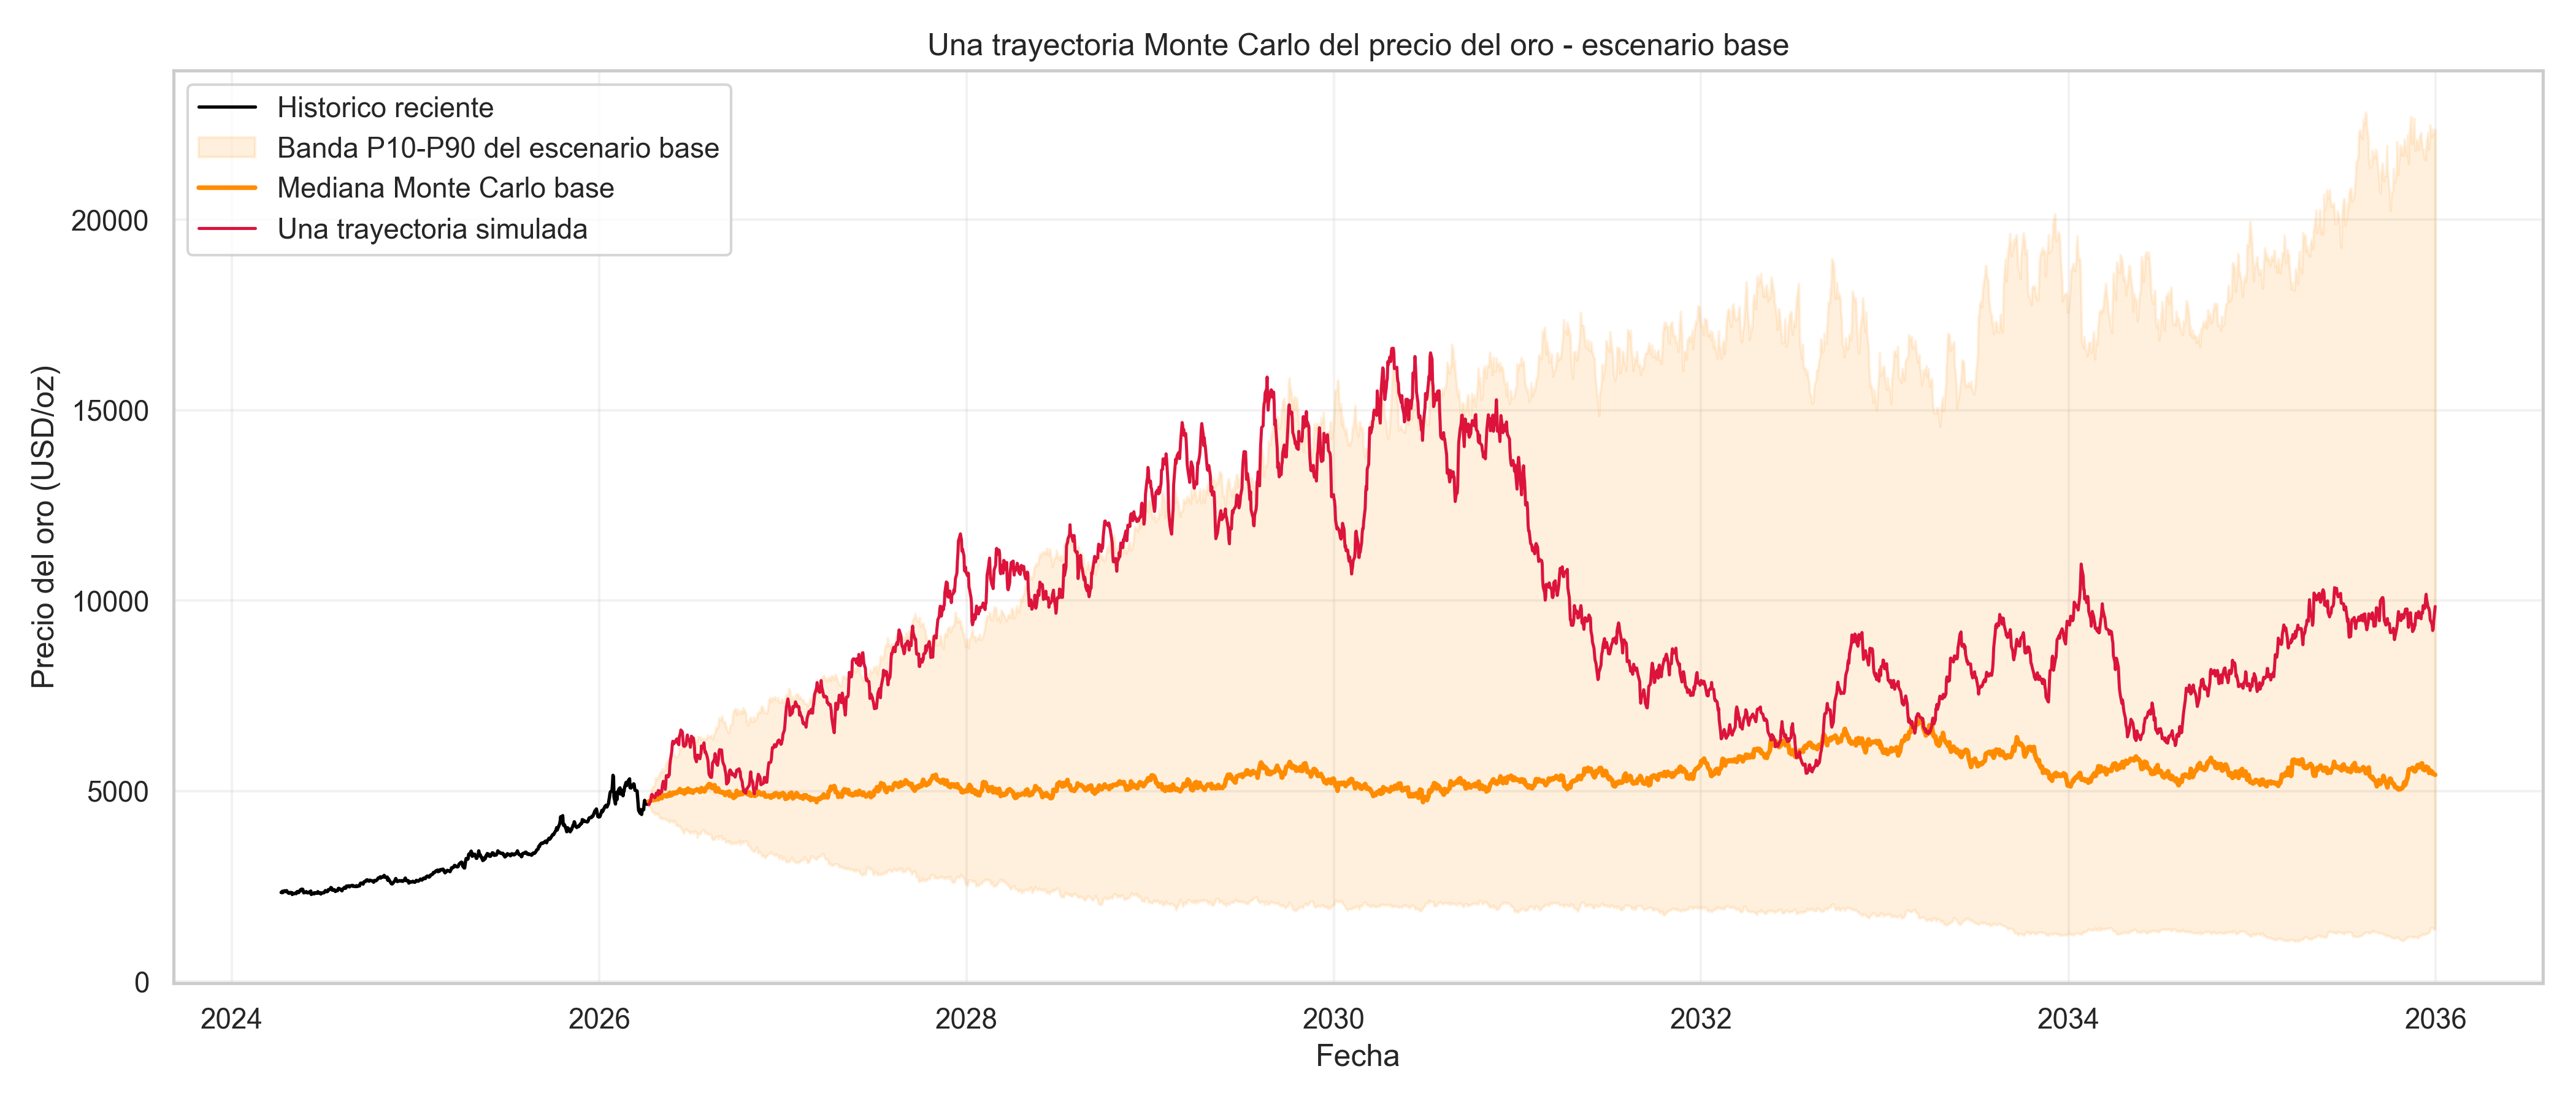
\includegraphics[width=0.95\textwidth]{09_trayectoria_unica_monte_carlo_base.png}
\caption{Una trayectoria Monte Carlo del precio del oro bajo escenario base.}
\label{fig:trayectoria}
\end{figure}

\section{Interpretación}
La forma de la trayectoria se debe a cuatro componentes: el retorno base predicho por LightGBM + Optuna, la volatilidad histórica/residual, la persistencia de los choques y la posibilidad de saltos aleatorios. Por eso esta línea no debe interpretarse como el valor exacto esperado, sino como una posible ruta del precio. La mediana representa el centro de las simulaciones, mientras que la trayectoria individual muestra un caso específico dentro de la incertidumbre modelada.

Si en varios días consecutivos los choques son positivos, la trayectoria se separa hacia arriba de la mediana. Si los choques son negativos, cae hacia la parte baja de la banda. Si se mantiene dentro de $P10$ y $P90$, significa que se encuentra dentro del rango central generado por la mayoría de las simulaciones. Si sale de esa banda, representa un comportamiento menos común dentro de los supuestos del escenario.

\end{document}
